%%%%%%%%%%%%%%%%%%%%%%%%%%%%%%%%%%%%%%%%
% datoteka diploma-vzorec.tex
%
% vzorčna datoteka za pisanje diplomskega dela v formatu LaTeX
% na UL Fakulteti za računalništvo in informatiko
%
% vkup spravil Gašper Fijavž, december 2010
% množica popravkov v januarju, februarju marcu 2011
% verzija 29. marec 2011

\documentclass[a4paper, 12pt]{book}

\usepackage[utf8x]{inputenc}   % omogoča uporabo slovenskih črk kodiranih v formatu UTF-8 
\usepackage[slovene,english]{babel}    % naloži, med drugim, slovenske delilne vzorce
\usepackage[pdftex]{graphicx}  % omogoča vlaganje slik različnih formatov 
\usepackage{fancyhdr}          % poskrbi, na primer, za glave strani
\usepackage{amssymb}           % dodatni simboli
\usepackage{amsmath}           % eqref, npr.


\renewcommand{\baselinestretch}{1.3} % ustrezen razmik med vrsticami

%oznake strani
\renewcommand{\chaptermark}[1]%
{\markboth{\MakeUppercase{\thechapter.\ #1}}{}} \renewcommand{\sectionmark}[1]%
{\markright{\MakeUppercase{\thesection.\ #1}}} \renewcommand{\headrulewidth}{0.5pt} \renewcommand{\footrulewidth}{0pt} 
\fancyhf{}
\fancyhead[LE,RO]{\sl \thepage} \fancyhead[LO]{\sl \rightmark} \fancyhead[RE]{\sl \leftmark}

\newcommand{\BibTeX}{{\sc Bib}\TeX}

\newcommand{\autfont}{\Large}
\newcommand{\titfont}{\LARGE\bf}
\newcommand{\clearemptydoublepage}{\newpage{\pagestyle{empty}\cleardoublepage}}
\setcounter{tocdepth}{1}	      % globina kazala

% konstrukti
\newtheorem{izrek}{Izrek}[chapter]
%\newtheorem{trditev}{Trditev}[izrek]
\newenvironment{dokaz}{\emph{Dokaz.}\ }{\hspace{\fill}{$\Box$}}

\begin{document}
\selectlanguage{slovene}
\frontmatter
\setcounter{page}{1} %
\renewcommand{\thepage}{}       % preprecimo težave s številkami strani v kazalu 

%%%%%%%%%%%%%%%%%%%%%%%%%%%%%%%%%%%%%%%%
%naslovnica
 \thispagestyle{empty}%
   \begin{center}
    {\large\sc Univerza v Ljubljani\\%
      Fakulteta za računalništvo in informatiko}%
    \vskip 10em%
    {\autfont Anže Pečar\par}%
    {\titfont Vzorec diplomskega dela \par}%
    {\vskip 2em \textsc{DIPLOMSKO DELO\\[2mm] 
    UNIVERZITETNI ŠTUDIJSKI PROGRAM RAČUNALNIŠTVO IN INFORMATIKA}\par}%
    \vfill\null%
    {\large \textsc{Mentor}: doc.\ dr.  Matjaž Kukar\par}%
    {\vskip 2em \large Ljubljana 2011 \par}%
\end{center}
% prazna stran
\clearemptydoublepage

%%%%%%%%%%%%%%%%%%%%%%%%%%%%%%%%%%%%%%%%
%copyright stran
\thispagestyle{empty}
\vspace*{8cm}
{\small \noindent
Rezultati diplomskega dela so intelektualna lastnina avtorja in Fakultete za ra\-ču\-nal\-niš\-tvo in informatiko Univerze v Ljubljani. 
Za objavljanje ali izkoriščanje rezultatov di\-plom\-ske\-ga dela je potrebno pisno soglasje avtorja, Fakultete za ra\-ču\-nal\-niš\-tvo in 
informatiko ter mentorja.}
\footnote{V dogovorju z mentorjem lahko kandidat diplomsko delo s pripadajočo izvorno kodo izda tudi pod katero izmed alternativnih licenc, ki ponuja določen del pravic vsem: npr. Creative Commons, GNU GPL. V tem primeru na to mesto vstavite opis licence, na primer tekst \cite{licence}}


\begin{center} 
\mbox{}\vfill
\emph{Besedilo je oblikovano z urejevalnikom besedil \LaTeX.} 
\end{center}
% prazna stran
\clearemptydoublepage

%%%%%%%%%%%%%%%%%%%%%%%%%%%%%%%%%%%%%%%%
% stran 3 med uvodnimi listi
\noindent
Namesto te strani {\bf vstavite} original izdane teme diplomskega 
dela s podpisom mentorja in dekana ter žigom fakultete, ki ga diplomant
dvigne v študent\-skem referatu,  preden odda izdelek v vezavo!
Glej tudi sam konec Poglavja~\ref{ch2} na strani~\pageref{pp}.

% prazna stran
\clearemptydoublepage

%%%%%%%%%%%%%%%%%%%%%%%%%%%%%%%%%%%%%%%%
% izjava o avtorstvu
\vspace*{1cm}
\begin{center} 
{\Large \textbf{\sc Izjava o avtorstvu diplomskega dela}}
\end{center}

\vspace{1cm}
\noindent Spodaj podpisani Anže Pečar,
z vpisno številko \textbf{63060257}, sem avtor  diplomskega dela z naslovom:
   
\vspace{0.5cm}
\emph{Vzorec diplomskega dela}

\vspace{1.5cm}
\noindent S svojim podpisom zagotavljam, da:
\begin{itemize}
	\item sem diplomsko delo izdelal samostojno pod mentorstvom 
		doc.\ dr.\ Matjaža Kukarja,

	\item	so elektronska oblika diplomskega dela, naslov (slov., angl.), povzetek (slov., angl.) ter ključne besede (slov., angl.) identični s tiskano obliko diplomskega dela
	\item soglašam z javno objavo elektronske oblike diplomskega dela v zbirki ''Dela FRI''.
\end{itemize}

\vspace{1cm}
\noindent V Ljubljani, dne 11. januarja 2011 \hfill Podpis avtorja:

% prazna stran
\clearemptydoublepage

%%%%%%%%%%%%%%%%%%%%%%%%%%%%%%%%%%%%%%%%
% zahvala
\thispagestyle{empty}\mbox{}\vfill\null\it%
Na tem mestu zapišite, komu se zahvaljujete za izdelavo diplomske naloge. Pazite, da ne boste koga pozabili. Utegnil vam bo zameriti. Temu se da izogniti tako, da pozabite na celo zahvalo.
\rm\normalfont

% prazna stran
\clearemptydoublepage

%%%%%%%%%%%%%%%%%%%%%%%%%%%%%%%%%%%%%%%%
% posvetilo
\thispagestyle{empty}\mbox{}{\vskip0.20\textheight}\mbox{}\hfill\begin{minipage}{0.55\textwidth}%
Svoji dragi Nataščici.
\normalfont\end{minipage}
 
% prazna stran
\clearemptydoublepage

%%%%%%%%%%%%%%%%%%%%%%%%%%%%%%%%%%%%%%%%
% kazalo
\def\thepage{}% preprecimo tezave s stevilkami strani v kazalu 
\tableofcontents{}


% prazna stran
\clearemptydoublepage

%%%%%%%%%%%%%%%%%%%%%%%%%%%%%%%%%%%%%%%%
% povzetek 
\addcontentsline{toc}{chapter}{Povzetek}
\chapter*{Povzetek}
V vzorcu je predstavljen postopek priprave diplomskega dela z uporabo okolja \LaTeX. Vaš povzetek mora sicer vsebovati približno 100 besed, ta tukaj je odločno prekratek.
% prazna stran
\clearemptydoublepage

%%%%%%%%%%%%%%%%%%%%%%%%%%%%%%%%%%%%%%%%
% abstract
\selectlanguage{english}
\addcontentsline{toc}{chapter}{Abstract}
\chapter*{Abstract}
This sample document presents an approach to typesetting your BSc thesis using \LaTeX. A proper abstract should contain around 100 words which makes this one way too short.
\selectlanguage{slovene}
% prazna stran
\clearemptydoublepage

%%%%%%%%%%%%%%%%%%%%%%%%%%%%%%%%%%%%%%%%
\mainmatter
\setcounter{page}{1}
\pagestyle{fancy}

\chapter{Uvod}
Datoteka {\tt diploma.tex} na kratko opisuje, kako se pisanja diplomskega dela lotimo z uporabo programskega pateka \LaTeX. V tem dokumentu bomo predstavili nekaj njegovih prednosti in hib. Kar se slednjih tiče, mi pride na misel ena sama. Ko se srečamo z njim nam izgleda kot kislo jabolko, nismo prepričani, da bi želeli vanj ugrizniti. Lahko pa z njim pripravimo odličen zavitek ali pa pridemo na okus.

Česa od tega dokumenta ne pričakujte? Izkušeni uporabniki \LaTeX{}a bi vse skupaj zastavili 
drugače. Morda bi napisali posebno razredno datoteko (\emph{class file}) --- v resnici priredili katero od obstoječih ---, v datoteki {\tt diploma.tex} ohranili samo najbolj grobo strukturo in vanjo vključevali  posamezna po\-glav\-ja. Hkrati s pisanjem teksta bi poskrbeli tudi za stvarno kazalo ({\tt makeindex}), literaturo pa bi citirali z uporabo {\BibTeX}{a}. Tega, skratka, v tem dokumentu ne boste našli.

Kaj vseeno najdemo. V Poglavju~\ref{ch1} bomo na hitro spoznali besedilne konstrukte kot so izreki, enačbe in dokazi. Naučili se bomo, kako se na njih sklicujemo. Poglavje~\ref{ch2} bo predstavilo vključevanje plovk: slik in tabel. V Poglavju~\ref{ch3} se bomo srečali s sklicevanjem na literaturo.
Sledil bo samo še zaključek.

\chapter{Sklicevanje na besedilne konstrukte}
\label{ch1}
Matematična ali popolna indukcija je eno prvih orodij, ki jih spoznamo za dokazovanje trditev pri matematičnih predmetih. 
\begin{izrek}
\label{iz:1}
Za vsako naravno število $n$ velja
\begin{equation}
n < 2^n.
\label{eq:1}
\end{equation}
\end{izrek}
\begin{dokaz}
Dokazovanje z indukcijo zahteva, da neenakost~\eqref{eq:1} najprej preverimo za najmanjše naravno število --- $0$. Res, ker je $0 < 1 = 2^0$, je neenačba~\eqref{eq:1} za $n=0$ izpolnjena.

Sledi indukcijski korak. S predpostavko, da je neenakost~\eqref{eq:1} veljavna pri nekem naravnem številu $n$, je potrebno pokazati, da je ista neenakost v veljavi tudi pri njegovem nasledniku --- naravnem številu $n+1$. Računajmo.
\begin{align}
n+1 &< 2^n + 1  \label{eq:2}\\
    &\le 2^n + 2^n \label{eq:3}\\
    &= 2^{n+1} \nonumber
\end{align} 
Neenakost~\eqref{eq:2} je posledica indukcijske predpostavke, neenakost~\eqref{eq:3} pa enostavno dejstvo, da je za vsako naravno število $n$ izraz $2^n$ vsaj tako velik kot 1. S tem je dokaz Izreka~\ref{iz:1} zaključen.
\end{dokaz}

Opazimo, da je \LaTeX\ številko izreka podredil številki poglavja.


\chapter{Plovke: slike in tabele}
\label{ch2}
Slike in daljše tabele praviloma vključujemo v dokument kot plovke. Pozicija plovke v končnem izdelku ni pogojena s tekom besedila, temveč z izgledom strani. \LaTeX\ bo skušal plovko postaviti samostojno, praviloma na vrh strani, na kateri se na takšno plovko prvič sklicujemo. Pri tem pa bo na vsako stran končnega izdelka želel postaviti tudi sorazmerno velik del besedila. V skrajnem primeru, če imamo res preveč plovk, se bo odločil za stran popolnoma zapolnjeno s plovkami.

\section{Formati slik}
Bitne slike, vektorske slike, kakršnekoli slike, z \LaTeX{}om lahko vključimo vse. 
Slika~\ref{pic1} je v {\tt .pdf} formatu.
\begin{figure}
\begin{center}
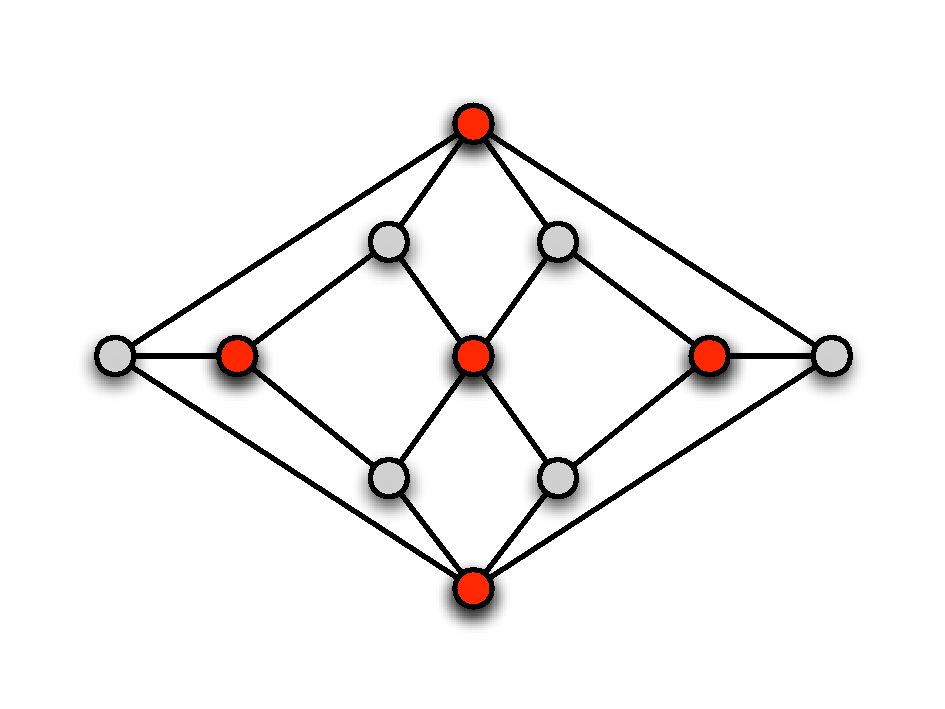
\includegraphics[width=10cm]{pic1.pdf}
\end{center}
\caption{Herschelov graf, vektorska grafika.}
\label{pic1}
\end{figure}
Pa res lahko vključimo slike katerihkoli formatov? Žal ne. Programski paket \LaTeX\ lahko uporabljamo v več dialektih. Ukaz {\tt latex} ne mara vključenih slik v formatu Portable Document Format {\tt .pdf}, ukaz {\tt pdflatex} pa ne prebavi slik v Encapsulated Postscript Formatu {\tt .eps}. 
Strnjeno v Tabeli~\ref{tbl:1}.

\begin{table}
\begin{center}
\begin{tabular}{l|ccc}
ukaz/format & {\tt .pdf} & {\tt .eps} & ostali formati \\ \hline
{\tt pdflatex} & da & ne & da \\
{\tt latex}   & ne & da  & da
\end{tabular}
\end{center}
\caption{}
\label{tbl:1}
\end{table}

Nasvet? Odločite se za uporabo ukaza {\tt pdflatex}. Vaš izdelek bo brez vmesnih stopenj na voljo v {.pdf} formatu in ga lahko odnesete v vsako tiskarno. Če morate na vsak način vključiti sliko, ki jo imate v {\tt .eps} formatu, jo vnaprej pretvorite v alternativni format, denimo {\tt .pdf}.

Včasih se da v okolju za uporabo programskega paketa \LaTeX\ nastaviti na kakšen način bomo prebavljali vhodne dokumente. Spustni meni na Sliki~\ref{pic2} odkriva uporabo \LaTeX{}a v njegovi pdf inkarnaciji --- {\tt pdflatex}.
\begin{figure}
\begin{center}
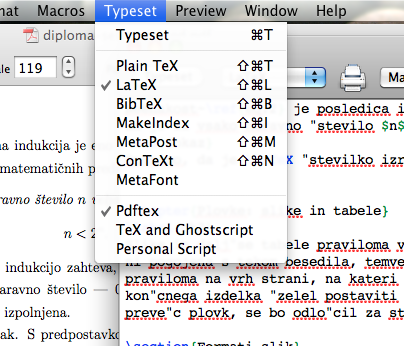
\includegraphics[width=10cm]{pic2.png}
\end{center}
\caption{Kateri dialekt uporabljati?}
\label{pic2}
\end{figure} 

Vključena Slika~\ref{pic2} je seveda bitna.

Kaj pa stran iz študentskega referata?\label{pp}
Tudi njo lahko vključimo v dokument. Toda ne kot plovko.
 

%\chapter{}

\chapter{Kaj pa literatura}
\label{ch3}
Kot smo omenili že v uvodu, je pravi način za citiranje literature uporaba \BibTeX{}a~\cite{bib}. 
Programski paket \LaTeX je prvotno predstavljen v priročniku~\cite{lat} in je v resnici nadgradnja sistema \TeX\ avtorja Donalda Knutha, znanega po denimo, če izpustim njegovo umetnost programiranja, Knuth-Bendixovem algoritmu~\cite{dk1}.

Vsem raziskovalcem s področja računalništva pa svetujem v branje mnenje L.\ Fortnowa~\cite{lf}.

\chapter{Sklepne ugotovitve}
Izbira \LaTeX\ ali ne \LaTeX\ je seveda prepuščena vam samim. Res je, da so prvi koraki v \LaTeX{}u težavni. Ta dokument naj vam služi kot začetna opora pri hoji.

\begin{thebibliography}{99}
\bibitem{lf} L.\ Fortnow, ``Viewpoint: Time for computer science to grow up'',
{\it Communications of the ACM}, št.\ 52, zv.\ 8, str.\ 33--35, 2009.
\bibitem{dk1} D.\ E.\ Knuth, P. Bendix. ``Simple word problems in universal algebras'', v zborniku: Computational Problems in Abstract Algebra (ur. J. Leech), 1970, str. 263--297.
\bibitem{lat} L.\ Lamport. {\it LaTEX: A Document Preparation System}. Addison-Wesley, 1986.
\bibitem{bib} O.\ Patashnik (1998) \BibTeX{}ing. 
Dostopno na:\\ http://ftp.univie.ac.at/packages/tex/biblio/bibtex/contrib/doc/btxdoc.pdf
\bibitem{licence} licence-cc.pdf. Dostopno na: 
\end{thebibliography}
\end{document}

